
\documentclass{bredelebeamer}

\usepackage{listings}
\usepackage{graphicx}
\usepackage{verbatim}


%%%%%%%%%%%%%%%%%%%%%%%%%%%%%%%%%%%%%%%%%%%%%%%%


\newcommand{\container}{\textit{container }}
\newcommand{\containers}{\textit{containers }}


\title[Seminario de Arquitecturas de Sistemas Distribuidos]{Avance de proyecto: Análisis de seguridad de Docker}
% Titre du diaporama

% Sous-titre optionnel

\author{Maximiliano Osorio}


\institute[UTFSM]
{
}


\date{}
% Optionnel. La date, généralement celle du jour de la conférence

% C'est utilisé dans les métadonnes du PDF



%\logo{
%
\includegraphics[scale=0.15]{images/logo.png}
%}



%%%%%%%%%%%%%%%%%%%%%%%%%%%%%%%%%%%%%%%%%%%%%%%%%%%%%%%%%%%%%%%%%%%%%
\begin{document}
\nocite{*}
\begin{frame}
  \titlepage
\end{frame}



\begin{frame}{Agenda}
  \tableofcontents
\end{frame}

%%%%%% Licence%%%%%%%%%%%%%%%%%%%%%%%%%%%%%%%%%%%%%%%%%%%%%%%%%%%%%%%%%%
% la classe LaTeX Bredelebeamer est placée sous licence GNU-GPL v3
% copyright 2015 Christophe Masutti
% https://github.com/framatophe/
% Il s'agit d'un style simple aux couleurs de Framasoft (http://framasoft.org)
% agrémenté de quelques boites.
%%%%%%%%%%%%%%%%%%%%%%%%%%%%%%%%%%%%%%%%%%%%%%%%%%%%%%%%%%%%%%%%%%%%%%%%


\NeedsTeXFormat{LaTeX2e}
\ProvidesClass{bredelebeamer}[17/02/2015, v1.0]

\PassOptionsToPackage{svgnames}{xcolor}
\LoadClass[compress,8pt]{beamer}





\usepackage[frenchb]{babel}
\usepackage[utf8]{inputenc}
\usepackage[T1]{fontenc}
\usepackage{helvet}
\usepackage{pdfpages}
\usepackage{graphicx}% http://ctan.org/pkg/graphicx
\usepackage[footnotesize,hang]{caption} % réduire la taille des légendes des images
\usepackage{hyperref}
\usepackage{tikz}










%%%% Les Framacouleurs

\definecolor{Framableu}{RGB}{12,91,122}
\definecolor{Framableulight}{RGB}{18,144,176}
\definecolor{Framavert}{RGB}{142,156,72}
\definecolor{Framavertlight}{RGB}{227,235,199}
\definecolor{Framarouge}{RGB}{204,45,24}
\definecolor{Framarougelight}{RGB}{249,189,187}
\definecolor{Framaviolet}{RGB}{106,86,135}
\definecolor{Framavioletlight}{RGB}{211,197,232}
\definecolor{Framaorange}{RGB}{235,114,57}
\definecolor{Framaorangelight}{RGB}{235,209,197}
\definecolor{Framajaune}{RGB}{196,168,27}
\definecolor{Framajaunelight}{RGB}{255,235,181}
\definecolor{Framamarron}{RGB}{161,136,127}
\definecolor{Framamarronlight}{RGB}{215,204,200}
\definecolor{Framagris}{RGB}{97,97,97}
\definecolor{Framagrislight}{RGB}{245,245,245}



%%%%%%%%%%%% Tableaux
\usepackage{tcolorbox}
\usepackage{tabularx}
\usepackage{array}
\usepackage{colortbl}
\tcbuselibrary{skins}


%%%% Merci : http://tex.stackexchange.com/questions/112343/beautiful-table-samples


\newcolumntype{Y}{>{\raggedleft\arraybackslash}X}

\tcbset{tabrouge/.style={enhanced,arc=0em,fonttitle=\bfseries,fontupper=\normalsize\sffamily,
colback=Framarougelight!100!white,colframe=Framarouge!70!black,colbacktitle=Framarouge!100!white,
coltitle=white,center title}}

\tcbset{taborange/.style={enhanced,arc=0em,fonttitle=\bfseries,fontupper=\normalsize\sffamily,
colback=Framaorangelight!100!white,colframe=Framaorange!70!black,colbacktitle=Framaorange!100!white,
coltitle=white,center title}}

\tcbset{tabvert/.style={enhanced,arc=0em,fonttitle=\bfseries,fontupper=\normalsize\sffamily,
colback=Framavertlight!100!white,colframe=Framavert!70!black,colbacktitle=Framavert!100!white,
coltitle=white,center title}}

\tcbset{tabbleu/.style={enhanced,arc=0em,fonttitle=\bfseries,fontupper=\normalsize\sffamily,
colback=Framableulight!100!white,colframe=Framableu!70!black,colbacktitle=Framableu!100!white,
coltitle=white,center title}}

\tcbset{tabjaune/.style={enhanced,arc=0em,fonttitle=\bfseries,fontupper=\normalsize\sffamily,
colback=Framajaunelight!100!white,colframe=Framajaune!70!black,colbacktitle=Framajaune!100!white,
coltitle=white,center title}}

\tcbset{tabgris/.style={enhanced,arc=0em,fonttitle=\bfseries,fontupper=\normalsize\sffamily,
colback=Framagrislight!100!white,colframe=Framagris!70!black,colbacktitle=Framagris!100!white,
coltitle=white,center title}}

\tcbset{tabmarron/.style={enhanced,arc=0em,fonttitle=\bfseries,fontupper=\normalsize\sffamily,
colback=Framamarronlight!100!white,colframe=Framamarron!70!black,colbacktitle=Framamarron!100!white,
coltitle=white,center title}}


%%%%%%%%%%%%%%%%%%%%%%%%%%%%%%%%%%%%%%%%%%%%%%%%%%









\beamerboxesdeclarecolorscheme{orange}{Framaorange}{Framaorangelight}



\usecolortheme[named=Framableu]{structure}

\useinnertheme{rectangles}
\useoutertheme[subsection=false]{miniframes}
\setbeamertemplate{navigation symbols}{}

\definecolor{sectionColor}{RGB}{0,0,0} % noir
\definecolor{subsectionColor}{RGB}{97,97,97} % Framagris
\definecolor{sectionTextColor}{RGB}{255,255,255} % blanc
\definecolor{subsectionTextColor}{RGB}{255,255,255} % blanc
\definecolor{leftFootlineColor}{RGB}{0,0,0}% noir
\definecolor{middleFootlineColor}{RGB}{97,97,97} % Framagris
\definecolor{rightFootlineColor}{RGB}{0,0,0}% noir
\definecolor{authorColor}{RGB}{255,255,255}% blanc
\definecolor{footlineTitleColor}{RGB}{255,255,255}% blanc
\definecolor{instituteColor}{RGB}{0,0,0}% noir
\definecolor{dateColor}{RGB}{255,255,255}% blanc
\definecolor{pageColor}{RGB}{255,255,255}% blanc
\definecolor{titleColor}{RGB}{12,91,122} % Framableu
\definecolor{titleTextColor}{RGB}{255,255,255} % blanc
\definecolor{bodyColor}{RGB}{255,255,255} % blanc
\definecolor{normalTextColor}{RGB}{0,0,0} % noir
\definecolor{exampleTextColor}{RGB}{82,99,42} %Framavertfoncé
\definecolor{alertTextColor}{RGB}{204,45,24} % Framarouge

\definecolor{chipColor}{RGB}{12,91,122} % Framableu
\definecolor{chipTextColor}{RGB}{255,255,255} % blanc
\definecolor{normalBlockColor}{RGB}{178,213,219} % Framableulight pour arriere plan du block
\definecolor{normalTitleBlockColor}{RGB}{12,91,122} % Framableu
\definecolor{normalBlockTextColor}{RGB}{0,0,0} % noir
\definecolor{normalBlockTitleTextColor}{RGB}{255,255,255} % blanc
\definecolor{exampleBlockColor}{RGB}{227,235,199} %Framavertlight pour arriere plan du block
\definecolor{exampleTitleBlockColor}{RGB}{142,156,72} % Framavert
\definecolor{exampleBlockTextColor}{RGB}{0,0,0} % noir
\definecolor{exampleBlockTitleTextColor}{RGB}{255,255,255} % blanc
\definecolor{alertBlockColor}{RGB}{249,189,187} % Framarougelight pour arriere plan du block
\definecolor{alertTitleBlockColor}{RGB}{204,45,24} % Framarouge
\definecolor{alertBlockTextColor}{RGB}{0,0,0} % noir
\definecolor{alertBlockTitleTextColor}{RGB}{255,255,255} % blanc


\setbeamertemplate{blocks}[rectangle]

\setbeamercolor{section in head/foot}{bg=sectionColor, fg=sectionTextColor}
\setbeamercolor{subsection in head/foot}{bg=subsectionColor, fg=subsectionTextColor}
\setbeamercolor*{block title}{fg=normalBlockTitleTextColor,bg=normalTitleBlockColor}
\setbeamercolor*{block body}{fg=normalBlockTextColor,bg=normalBlockColor}
\setbeamercolor*{block title alerted}{fg=alertBlockTitleTextColor,bg=alertTitleBlockColor}
\setbeamercolor*{block body alerted}{fg=alertBlockTextColor,bg=alertBlockColor}
\setbeamercolor*{block title example}{fg=exampleBlockTitleTextColor,bg=exampleTitleBlockColor}
\setbeamercolor*{block body example}{fg=exampleBlockTextColor,bg=exampleBlockColor}
\setbeamerfont{block title}{size={}}
\setbeamercolor{titlelike}{fg=titleTextColor,bg=titleColor}
\setbeamercolor*{normal text}{fg=normalTextColor,bg=bodyColor}
\setbeamercolor*{example text}{fg=exampleTextColor}
\setbeamercolor*{alerted text}{fg=alertTextColor}
\setbeamercolor{itemize item}{fg=titleColor!70}
\setbeamercolor{enumerate item}{fg=titleColor!70}
\setbeamercolor{description item}{fg=titleColor!70}


\useinnertheme{default}
\setbeamercolor{item projected}{bg=chipColor,fg=chipTextColor}
\beamer@compresstrue
\defbeamertemplate*{headline}{smoothbars theme}
{%
\begin{beamercolorbox}[ht=2.125ex,dp=3.150ex]{section in head/foot}
\insertnavigation{\paperwidth}
\end{beamercolorbox}%

% Commenter les 4 lignes suivantes si vous ne voulez pas la barre des sous-sections.
\begin{beamercolorbox}[ht=2.125ex,dp=1.125ex,%
leftskip=.3cm,rightskip=.3cm plus1fil]{subsection in head/foot}
\usebeamerfont{subsection in head/foot}\insertsubsectionhead
\end{beamercolorbox}%
}
\setbeamercolor{author in head/foot}{bg=leftFootlineColor, fg=authorColor}
\setbeamercolor{title in head/foot}{bg=middleFootlineColor, fg=footlineTitleColor}
\setbeamercolor{institute in head/foot}{fg=instituteColor}
\setbeamercolor{date in head/foot}{bg=rightFootlineColor, fg=dateColor}
\defbeamertemplate*{footline}{infolines theme}
{
\leavevmode%
\hbox{%
\begin{beamercolorbox}[wd=.333333\paperwidth,ht=2.25ex,dp=1ex,center]{author in head/foot}%
\usebeamerfont{author in head/foot}\insertshortauthor~~
\insertshortinstitute
\end{beamercolorbox}%
\begin{beamercolorbox}[wd=.333333\paperwidth,ht=2.25ex,dp=1ex,center]{title in head/foot}%
\usebeamerfont{title in head/foot}\insertshorttitle
\end{beamercolorbox}%
\begin{beamercolorbox}[wd=.333333\paperwidth,ht=2.25ex,dp=1ex,right]{date in head/foot}%
\usebeamerfont{date in head/foot}\insertshortdate{}\hspace*{2em}
\insertframenumber{} / \inserttotalframenumber\hspace*{2ex}
\end{beamercolorbox}
}%
\vskip0pt%
}
\mode
<all>

%utilise la couleur Beamer : "example text" pour la couleur du texte
\newcommand{\exemple}[1]{{\color{example text.fg} #1}}

% emphase
\renewcommand{\emph}[1]{\textcolor{Framaorange}{\textbf{#1}}}


\usepackage{etoolbox}
\AtBeginEnvironment{exampleblock}{%
  \setbeamercolor{itemize item}{fg=exampleTitleBlockColor!70}
}
\AtBeginEnvironment{alertblock}{%
  \setbeamercolor{itemize item}{fg=alertTitleBlockColor!70}
}
\AtBeginEnvironment{block}{%
  \setbeamercolor{itemize item}{fg=normalTitleBlockColor!70}
}


\newcommand{\boitejaune}[1]{
\begin{center}
\fcolorbox{Framajaune}{Framajaunelight}{
\begin{minipage}{0.5\textwidth}
#1
\end{minipage}
}
\end{center}
}


\newcommand{\boiteviolette}[1]{
\begin{center}
\fcolorbox{Framaviolet}{Framavioletlight}{
\begin{minipage}{0.5\textwidth}
#1
\end{minipage}
}
\end{center}
}


\newcommand{\boiteorange}[1]{
\begin{center}
\fcolorbox{Framaorange}{Framaorangelight}{
\begin{minipage}{0.5\textwidth}
#1
\end{minipage}
}
\end{center}
}


\newcommand{\boitemarron}[1]{
\begin{center}
\fcolorbox{Framamarron}{Framamarronlight}{
\begin{minipage}{0.5\textwidth}
#1
\end{minipage}
}
\end{center}
}

\newcommand{\boitegrise}[1]{
\begin{center}
\fcolorbox{Framagris}{Framagrislight}{
\begin{minipage}{0.5\textwidth}
#1
\end{minipage}
}
\end{center}
}


\newcommand{\boitebleue}[1]{
\begin{center}
\fcolorbox{Framableu}{Framableulight}{
\begin{minipage}{0.5\textwidth}
#1
\end{minipage}
}
\end{center}
}



\section{Motivación y descripción del problema}
	

\begin{frame}{Motivación}
	\begin{figure}
		\centering
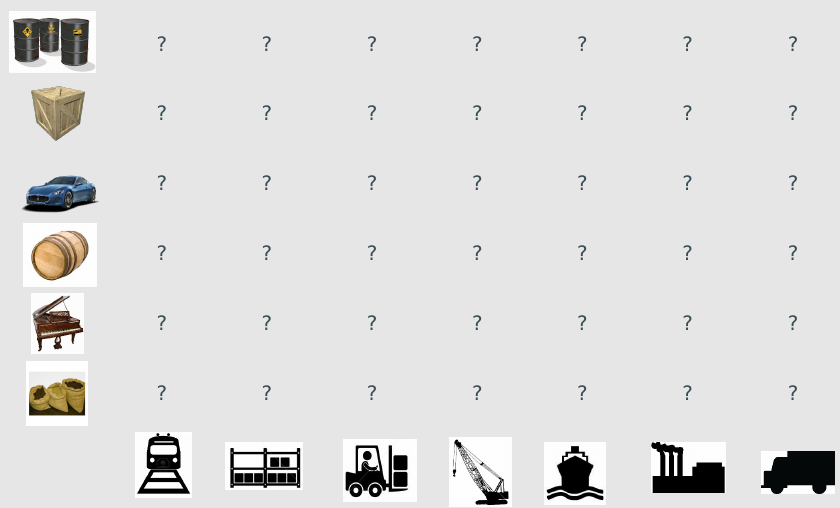
\includegraphics[width=\textwidth,height=0.8\textheight,keepaspectratio]{images/another}
	\end{figure}
\end{frame}

\begin{frame}{Motivación}
	\begin{figure}
		\centering
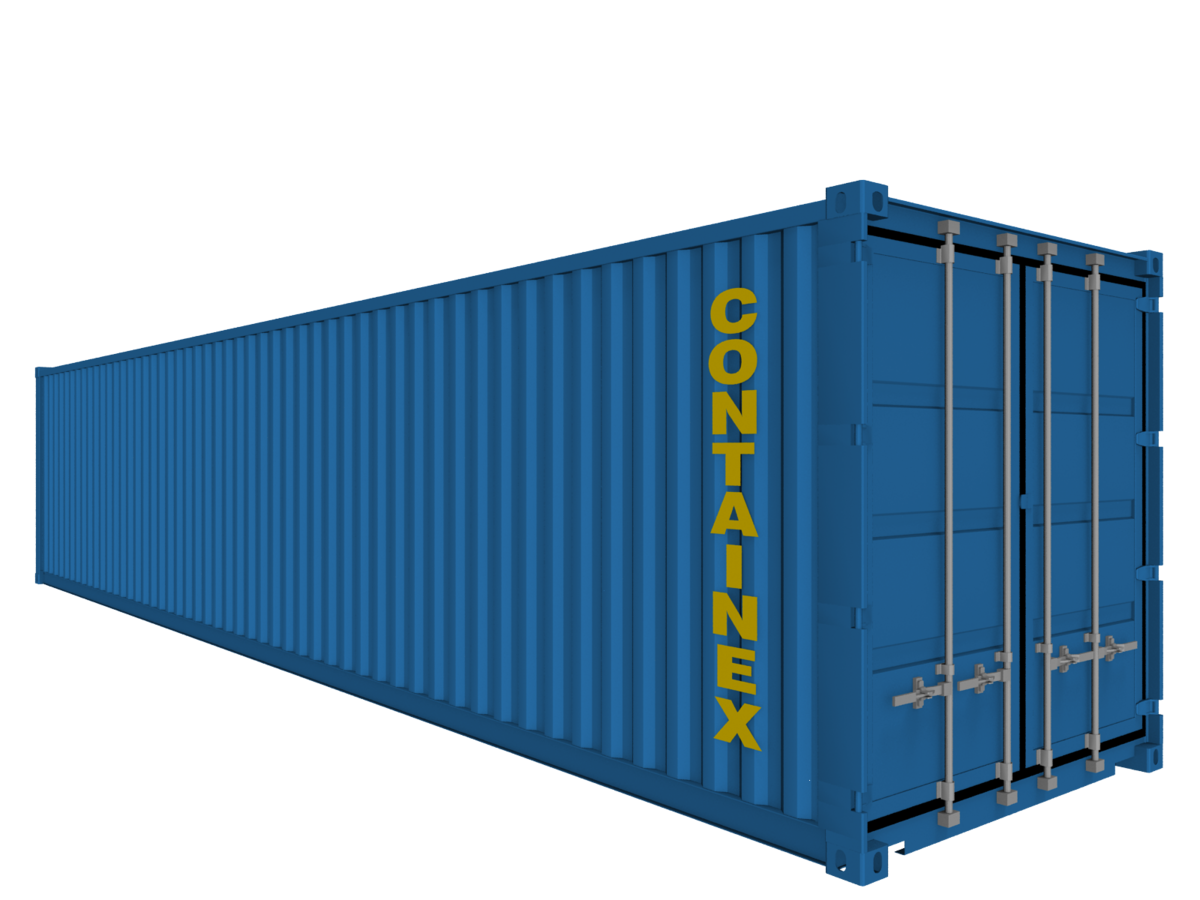
\includegraphics[width=\textwidth,height=0.8\textheight,keepaspectratio]{images/r_container}
	\end{figure}
\end{frame}


\begin{frame}{Motivación}
	\begin{figure}
		\centering
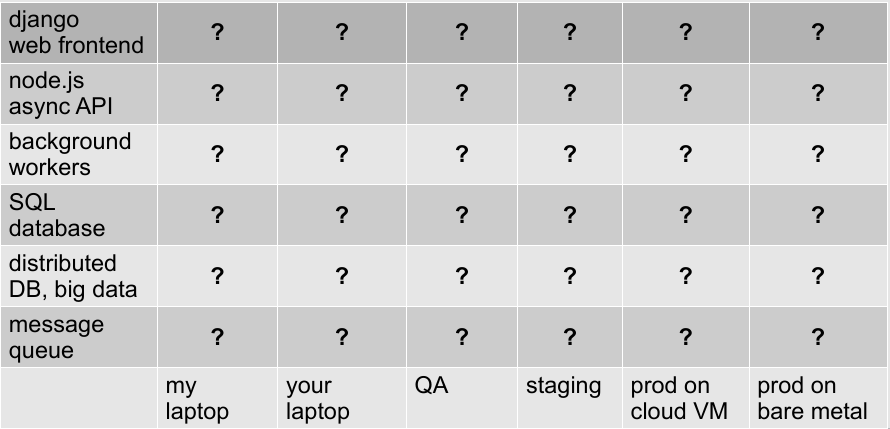
\includegraphics[width=\textwidth,height=0.8\textheight,keepaspectratio]{images/matrix}
		\caption{Representation flow shop scheduling problem. (\href{http://yetanothermathprogrammingconsultant.blogspot.com/2012_04_01_archive.html} CC-By-Sa)}
	\end{figure}
\end{frame}


\begin{frame}{Motivación}
	\begin{figure}
		\centering
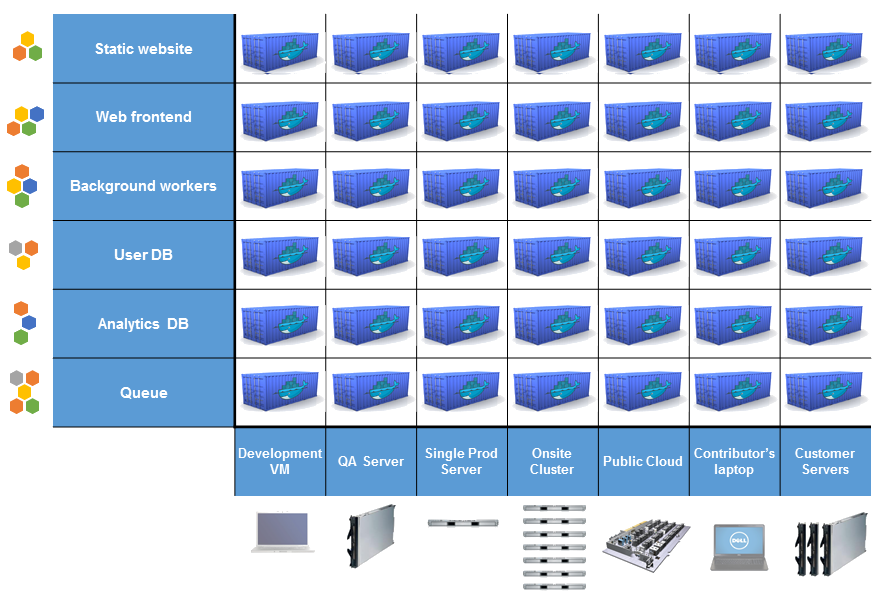
\includegraphics[width=\textwidth,height=0.8\textheight,keepaspectratio]{images/eliminates-matrix-from-hell}
		\caption{Representation flow shop scheduling problem. (\href{http://yetanothermathprogrammingconsultant.blogspot.com/2012_04_01_archive.html} CC-By-Sa)}
	\end{figure}
\end{frame}

\begin{frame}{Motivación}
	\begin{figure}
		\centering
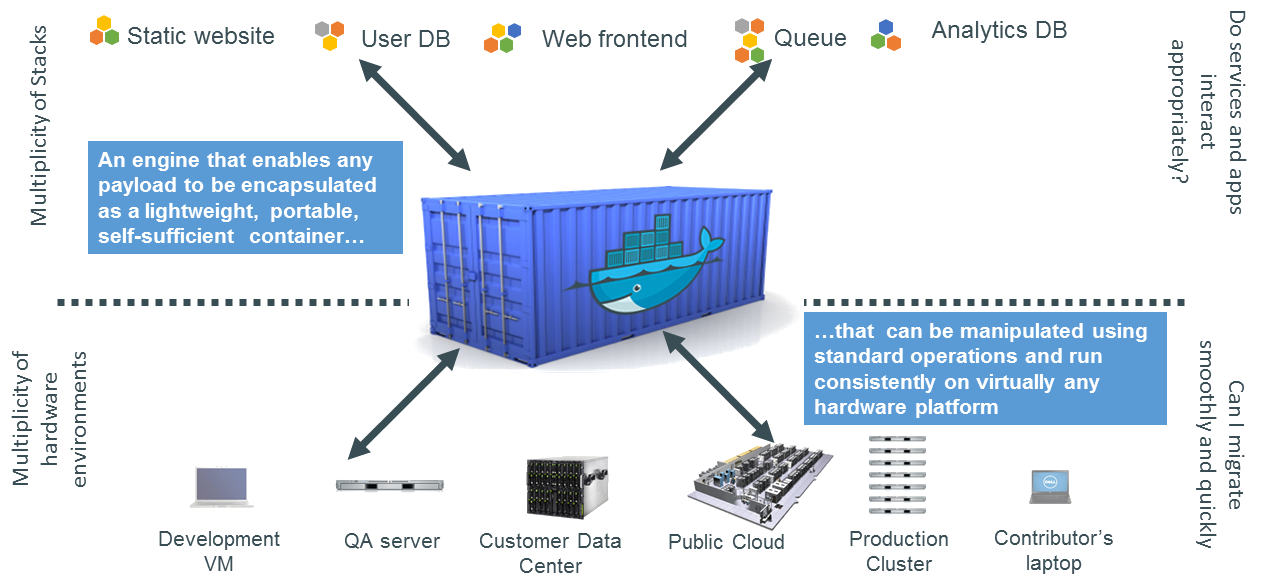
\includegraphics[width=\textwidth,height=0.8\textheight,keepaspectratio]{images/shipping-container-for-code}
		\caption{Representation flow shop scheduling problem. (\href{http://yetanothermathprogrammingconsultant.blogspot.com/2012_04_01_archive.html} CC-By-Sa)}
	\end{figure}
\end{frame}

\begin{frame}{Docker}
	\begin{itemize}
		\item 	Docker es un proyecto open-source que utiliza la tecnología de los containers (libcontainer) para ``construir, migrar y correr aplicaciones distribuidas". Los containers se basan en \textit{container-based virtualization} 
		\item ¿Qué son los containers?
			\begin{itemize}
				\item Desde lejos, parecen ser como VM.
				\item Puedo instalar aplicaciones, tengo root, tengo red, montar filesystems, etc.
				\item Pero son ambientes virtuales livianos, rápidos de iniciar (boot en ms), facil de migrar, deterministas y otros.
			\end{itemize}
	\end{itemize}

\end{frame}


\begin{frame}{¿Problema?}
	
¿Es seguro correr aplicaciones en Linux Containers?
\end{frame}



\begin{frame}
	\begin{figure}
		\centering
		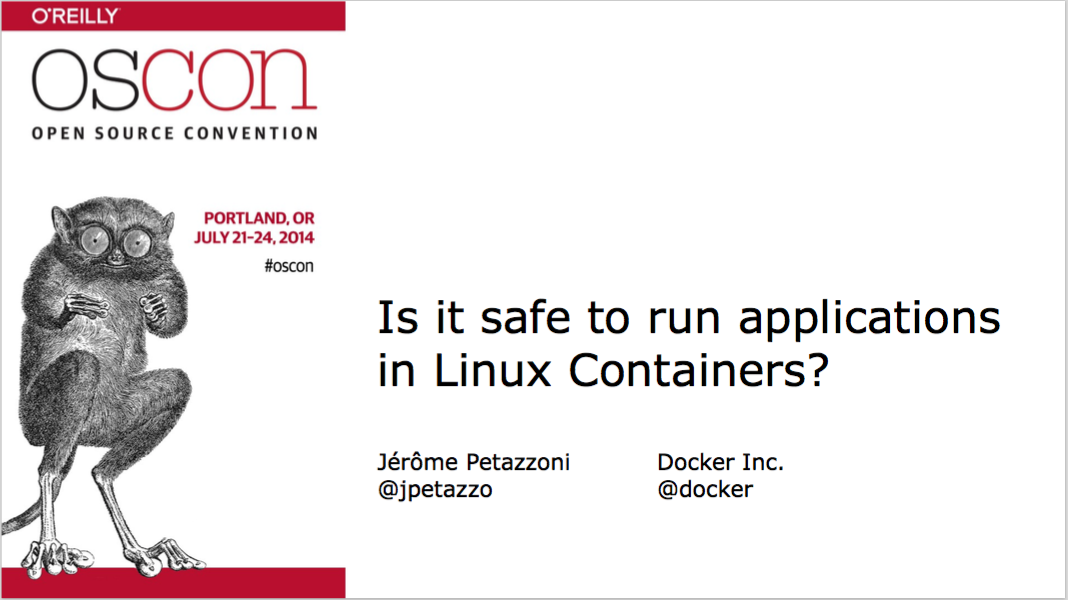
\includegraphics[width=\textwidth,height=0.8\textheight,keepaspectratio]{images/oscon1}
		\caption{De: Jerome Petazzoni, Docker}
	\end{figure}
\end{frame}
\begin{frame}
	\begin{figure}
		\centering
		
\includegraphics[width=\textwidth,height=0.8\textheight,keepaspectratio]{images/oscon2}
		\caption{De: Jerome Petazzoni, Docker}
	\end{figure}
\end{frame}
\begin{frame}
	\begin{figure}
		\centering
		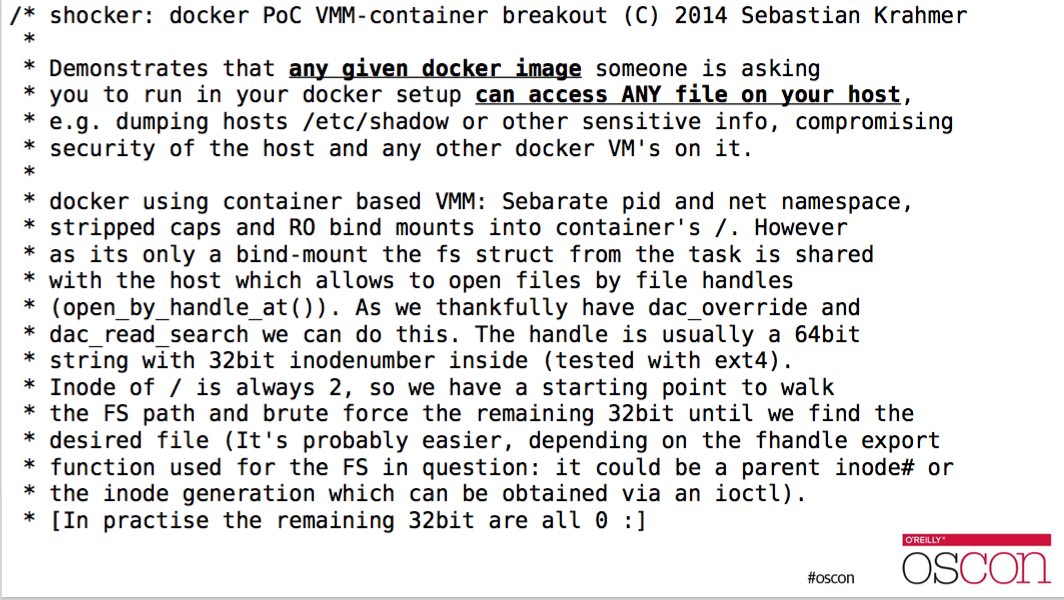
\includegraphics[width=\textwidth,height=0.8\textheight,keepaspectratio]{images/oscon3}
		\caption{De: Jerome Petazzoni, Docker}
	\end{figure}
\end{frame}
\begin{frame}
	\begin{figure}
		\centering
		
\includegraphics[width=\textwidth,height=0.8\textheight,keepaspectratio]{images/oscon4}
		\caption{De: Jerome Petazzoni, Docker}
	\end{figure}
\end{frame}
\begin{frame}
	\begin{figure}
		\centering
		
\includegraphics[width=\textwidth,height=0.8\textheight,keepaspectratio]{images/oscon5}
		\caption{De: Jerome Petazzoni, Docker}
	\end{figure}
\end{frame}

\begin{frame}
	\begin{figure}
		\centering
		
\includegraphics[width=\textwidth,height=0.8\textheight,keepaspectratio]{images/oscon6}
		\caption{De: Jerome Petazzoni, Docker}
	\end{figure}
\end{frame}


\begin{frame}{Agenda}
  \tableofcontents
\end{frame}

\section{Avances}
\subsection{Marco teorico}

\begin{frame}{Componentes}
	
	\begin{itemize}
		\item Docker registry
		\item Docker client
		\item Docker
		\begin{itemize}
			\item Docker Images
			\item Docker Containers
		\end{itemize}

	\end{itemize}
\end{frame}


\begin{frame}{Docker registry}
\begin{itemize}
	\item Repositorios públicos (Docker Hub) y privados de imágenes.
	\item Permite subir y bajar imágenes con sistemas operativos o aplicaciones ya configuradas.
	\item Imágenes son verificadas autenticidad y integridad.	
	\item Son usadas para construir Docker containers.
\end{itemize}

\end{frame}

\begin{frame}{Docker image}
\begin{itemize}
	\item Template read-only que son obtenidas desde registry.
	\item Son usadas para construir Docker containers.
	\item Los cambios realizados se hacen a través de capas.
\end{itemize}
\begin{figure}[H]
  \centering
  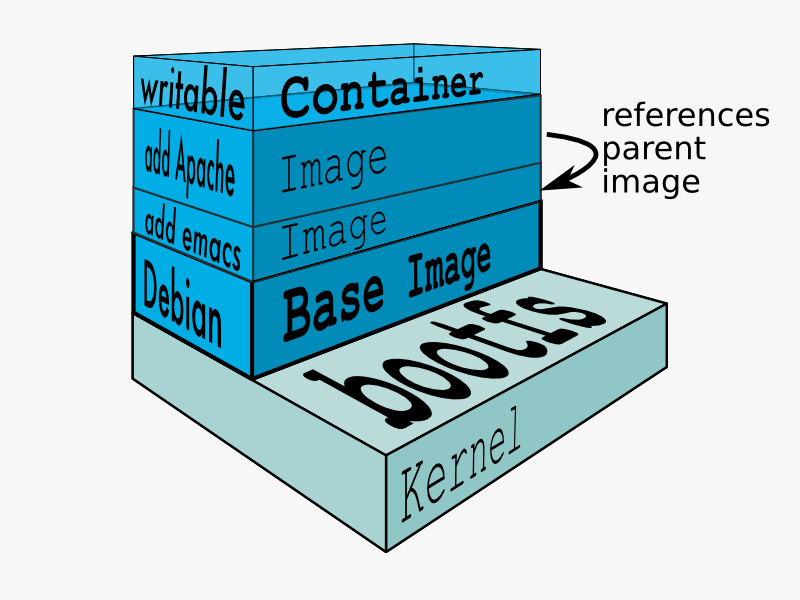
\includegraphics[width=0.6\textwidth]{images/docker-filesystems-multilayer}
    \caption{Representación \textit{union file system}}
    \label{fig:arquitectura}
\end{figure}	
\end{frame}

\begin{frame}{Docker registry}

\begin{figure}[H]
  \centering
  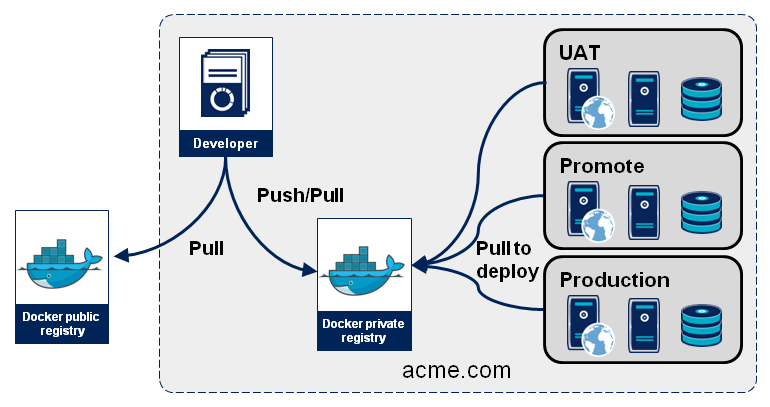
\includegraphics[width=\textwidth,height=0.8\textheight,keepaspectratio]{images/registry-dynamic.png}
    \caption{Representación \textit{Dinámica de un \textit{Docker registry} }}
    \label{fig:dynamic}
\end{figure}	
\end{frame}



\begin{frame}{Docker containers}
\begin{itemize}
	\item 	Docker \textit{container} consiste de  un sistema operativo, con archivos de usuarios y metadata.
	\item Es construido en base a la imagen.
\end{itemize}
\begin{block}{Ejemplo}
docker run -ti ubuntu /bin/bash
\end{block}

\end{frame}


\begin{frame}{Docker containers}
	\begin{itemize}
		\item \textit{Docker client} le informa al Docker que debe correr un \textit{container}.
		\item El comando \emph{/bin/bash} será el \textit{init 0} del container 
		\item \textbf{Traer la imagen:} Docker verifica la existencia de la imagen ubuntu y sino existe en el host, entonces Docker descarga de un \textit{registry} ya sea privado o publico. Si la imagen existe entonces crea el container.
		\item \textbf{Asignar un \emph{filesystem} y montar una capa \emph{read-write}:} El 
			container es creado en el \emph{filesystem} y se añade una capa en modo 
			\emph{read-write} a la imagen.
		\item \textbf{Crear la red y conectar con el \emph{bridge interface}:} Crea la interfaz de red que permite que el Docker container pueda hablar con el host a través del bridge (docker0).
		\item \textbf{Asignar un IP:} Asigna una ip del pool al container
		\item \textbf{Capturar el \textit{output}, \textit{input} y errores}.
	\end{itemize}
\end{frame}

\begin{frame}{Aislamiento}
	\begin{itemize}
		\item \textbf{Limite de recursos:}  Cgroups controlan la cantidad de recursos como CPU, memoria y disk I/O 
		\item \textbf{Process:} Utiliza PID namespaces (kernel \(\geq 2.6.32\), el container solo puede ver los procesos del container.
		\item \textbf{Filesystem:} Mismo mecanismo y mismo resultado que con los procesos. Existen device que deben ser montados (ej. /sys).
		\item \textbf{Device:} Cgroups permite usar algunos devices \footnote{/dev/console, /dev/null, /dev/zero, /dev/full, /dev/tty*, /dev/urandom, /dev/random, /dev/fuse} y bloquea la posibilidad de crear y usar otros devices.
		\item \textbf{IPC:} Los procesos corriendo en los \containers utilizan \textit{IPC namespaces} que permite la creación de un \textit{IPC} separado y independiente para cada \container 

	\end{itemize}
\end{frame}

\begin{frame}{Aislamiento}
	\begin{itemize}
	
		\item \textbf{Network:}
		Para cada \container, Docker crea una red independiente usando \emph{network namespaces}, compuesta de su propia IP, rutas, \emph{network devices}.
		Por defecto, la conexión se realiza gracias al host que provee un \emph{Virtual Ethernet bridge} en la máquina, llamado docker0 que automaticamente realiza un \emph{forward} de los paquetes entre las interfaces del container.
	\end{itemize}
	
	\begin{figure}[H]
  \centering
  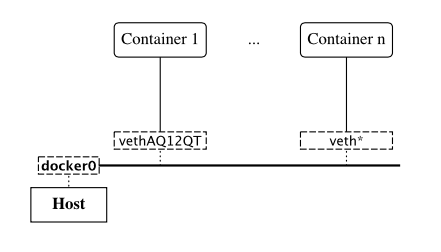
\includegraphics[width=0.5\textwidth]{images/network.png}
    \caption{Network}
    \label{fig:dynamic}
\end{figure}	
\end{frame}


\subsection{Implementación}


\begin{frame}{Ambiente de prueba}
	Actualmente la implementación base se encuentra lista. Utilizando un nodo
Centos con project-atomic y Docker 1.5.0. Se habilitó SElinux para
realizar pruebas con un \textit{Mandatory Access Control}

\begin{block}{Versión}
	Docker version 1.5.0, build a8a31ef/1.5.0

\end{block}
\end{frame}


\subsection{Discusión y posibles ataques}

\subsubsection{Secure image repository}
\begin{frame}{Secure image repository}
Basado en la idea de Fernandez, Monge y Hashizume  de \textit{Secure
virtual machine image repository} \cite{fernandez_monge:2015} se investigó sobre si Docker hub cumple con los patrones especificados.
 \begin{itemize}
 	\item Desde Docker \(\geq 1.3.0\) se completa las defensas descritas:  Authenticator-Authorizer, Secure Channel, Security Logger/Auditor y filter.
 	\item Rudenberg \cite{rudenberg:2015:Online} y Jay \cite{jay:2014:Online} alertan que el proceso de traer un imagen no es seguro. CVE-2014-9356, CVE-2014-9357, CVE-2014-9358 \cite{lvm-cve:2014:Online}
	\item Al probar realizar las pruebas, se determina que no afectan a la última versión de Docker.
 	
 \end{itemize}

	  
\end{frame}
\subsubsection{ARP-spoofing attack}

\begin{frame}{ARP-spoofing attack}

 \begin{itemize}
 	\item El modelo de red permite comunicación layer-2.
 	\item Por defecto los containers se pueden comunicar, aunque existe una opcion --icc que aisla al container de los otros (red).
 	\item --icc funciona a nivel de iptables (layer-3)
 \end{itemize}
 
 
 	\begin{figure}[H]
  \centering
  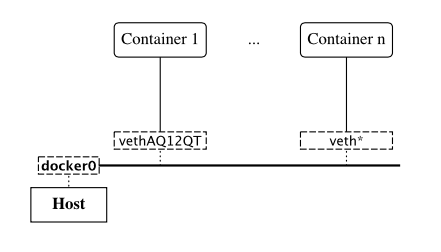
\includegraphics[width=0.5\textwidth]{images/network.png}
    \caption{Network}
    \label{fig:dynamic}
\end{figure}	
\end{frame}



\begin{frame}{Solución ARP-spoofing attack}
nyatec propone dos soluciones para esto: \cite{nyantec:2015:Online}.

 \begin{itemize}
 	\item Eliminar la capacidad 
de NET\_RAW para evitar que el \container puede crear \textit{PF\_PACKET sockets} 
que son necesarios para el ARP spoofing attack.
 	\item La utilización de etables para 
filtrar los \textit{Ethernet frame} con direcciones de destino incorrecto.
 \end{itemize}

La utilización de SElinux también es una solución comprobado en la prueba de concepto.
\end{frame}

	  

\section{Conclusiones preliminares}

\begin{frame}{Conclusiones preliminares}

\begin{itemize}
	\item Docker es un sistema seguro siendo utilizado con la configuración por defecto aunque si existen vulnerabilidades como se nombro anteriormente.
	\item Utilización de herramientas complementarías como SElinux aumentan el grado de seguridad.
\end{itemize}
\end{frame}


\section{Trabajo restante}


\begin{frame}{Trabajo restante}
	\begin{itemize}
	\item Completar investigación con \emph{Linux Capabilities} y \emph{Mandatory Access Control}
	\item Alcances de ataques en un ambiente de Docker con SElinux (MAC) integrado.
	\item Contestar la pregunta ¿Es posible asegurar el host o los \containers  si el atacante salió del \container?.
\end{itemize}
\end{frame}

\section{Referencias}
\begin{frame}[allowframebreaks]
\frametitle{Referencias}
\bibliographystyle{plain}
\bibliography{ref}
\end{frame}

\end{document}
